\title{Extending Programming Languages with Diagrammatic Programming Languages}
\documentclass{acmart}

\title{Extending Programming Languages with Diagrammatic Programming Languages}
\author{Zac Nowicki}
\affiliation{
  \institution{Kagi Inc.}
  \city{Palo Alto}
  \state{CA}
  \country{USA}
}
\email{znowicki@kagi.com}

\author{Paul Tarvydas}
\affiliation{
  \institution{Retired}
  \city{Toronto}
  \state{Ontario}
  \country{Canada}
}
\email{paultarvydas@gmail.com}

\begin{document}

\maketitle

\section{Abstract}
This paper describes a technique for extending the syntax of programming languages.

The new syntax consists of drawings containing simple, closed, graphical figures and arrows.

We use the name "DPL" - Diagrammatic Programming Languages - when referring to this class of new programming syntax.

We assert that DPLs might be used \emph{alongside} of existing TPLs (Textual Programming Languages) and that DPLs are hybrids of diagram and textual notations.

There are multiple possible DPL syntaxes. This paper suggests but a single DPL syntax. It is assumed that a variety of syntaxes might be invented, using the techniques described herein.

This paper touches on some of the key aspects of making compilable and understandable drawings of programs, e.g., 0D, syntactic simplicity, DI (Design Intent), etc.

We do not discuss fundamental DPL principles in this paper and refer the reader to other related writings on these subjects.

[TBD] This paper is laid out in XXX (???) sections.

\section{Example}
The above diagram is a motivating example.

The above diagram shows but one sample of a practical DPL syntax. Variations and improvements on this syntax can be imagined. The above syntax is being used to produce actual applications like term-rewriting (*t2t* text-to-text rewriting) compilers, LLMs, DSLs for creating DSLs, Visual Shell prototypes, games, etc.

This DPL syntax consists of only a few kinds of closed figures plus arrows plus text belonging to the closed figures. Everything else is considered to be a comment, and is ignored. For example, the bold text "Sequential Routing" is ignored. Colors are ignored. Line shapes and line widths are ignored, and so on.

This diagram was drawn using the off-the-shelf diagram editor \href{http://draw.io}{draw.io}\footnote{\url{http://draw.io}}. The editor saves the diagram in a modified form of XML, called \emph{graphML}\footnote{\url{https://en.wikipedia.org/wiki/GraphML}}.

The graphML file can be processed using off-the-shelf tools, like an XML parser or a PEG-based parser\footnote{\url{https://en.wikipedia.org/wiki/Parsing_expression_grammar}}\footnote{\url{http://ohmjs.org}}.

In our case, we used the Odin programming language\footnote{Odin} and the XML parsing library that is included in the Odin library\footnote{Odin XML parser}.

We choose not to reproduce the code for the actual diagram parser here, due to space limitations for this paper. The full source code for the functioning diagram parser is in an open-source repo\footnote{\url{https://github.com/guitarvydas/onward/tree/main/helloworld0d/0D/das2json}}.

The diagram parser produces internal data structures in the host programming language and/or JSON\footnote{JSON} files.

A \href{http://draw.io}{draw.io} file can contain several diagrams, each on a separate tab (window) in the editor.

The structure of the information needed by the DPL runtime is minimal, consisting of about four (4) fields for each diagram:

\begin{verbatim}
"file": "helloworld0d.drawio",
"name": "main",
"children": [
{
"name": "Echo",
"id": 6
},
... (2 more children referring to the same template "Echo", but assigned
Different ids) ...
],
"connections": [
{
"dir": 0,
"source": {
"name": "",
"id": 0
},
"source_port": "",
"target": {
"name": "Echo",
"id": 6
},
"target_port": ""
},
... [7 more connections as per the diagram] ...
]
\end{verbatim}

The filename of the \href{http://draw.io}{draw.io} drawing

The tab-name of the top-most diagram.

A bag of Children components.

A bag of Connections between children (including connections to/from the parent containing diagram).

\section{Compilation and Execution}

Compilation and execution of this DPL consists of the following steps:

\begin{enumerate}
  \item Convert DPL program diagrams to JSON

  \begin{figure}[h]
    \centering
    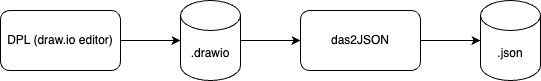
\includegraphics[width=0.8\linewidth]{./media/image2.png}
    \caption{Towards DPLs-1. Convert diagram to JSON}
    \label{fig:convert_to_json}
  \end{figure}

  Transpilation of the diagrams (XML) into JSON (or internal data structures, if efficiency is at a premium). The diagrams represent \emph{templates} for components.
  
  In our implementation, \texttt{das2json}\footnote{\url{https://github.com/guitarvydas/onward/tree/main/helloworld0d/0D/das2json}} is implemented\footnote{\url{https://github.com/guitarvydas/onward/tree/main/helloworld0d/0D/das2json}} in the Odin programming language. The process begins with a straightforward call to the XML parsing library. The XML data is then deconstructed into a convenient internal format (see \texttt{0d/ir/ir\_odin}).

  \item Load component templates from JSON

  \begin{figure}[h]
    \centering
    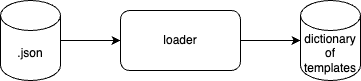
\includegraphics[width=0.6\linewidth]{./media/image3.png}
    \caption{Towards DPLs-2. Loader}
    \label{fig:load_templates}
  \end{figure}

  Ingestion of the JSON, or internal data structures into an internal database that we call a \emph{registry} (which can be implemented as a \emph{dictionary, map} or a \emph{database}).

  \item Instantiate system

  \begin{figure}[h]
    \centering
    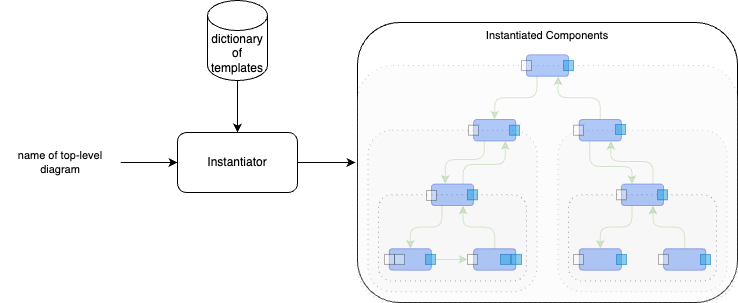
\includegraphics[width=0.8\linewidth]{./media/image4.png}
    \caption{Towards DPLs-3. Instantiate}
    \label{fig:instantiate_system}
  \end{figure}

  \item Inject first message

  \begin{figure}[h]
    \centering
    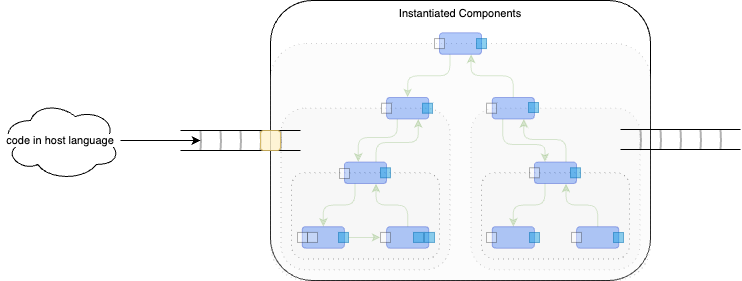
\includegraphics[width=0.8\linewidth]{./media/image5.png}
    \caption{Towards DPLs-4. Inject first message(s)}
    \label{fig:inject_first_message}
  \end{figure}

  \item Run

  \begin{figure}[h]
    \centering
    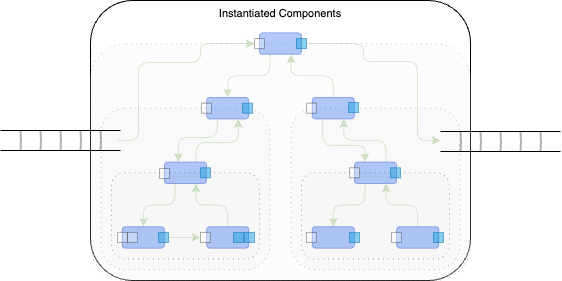
\includegraphics[width=0.8\linewidth]{./media/image6.png}
    \
